\title{INF564 Project report}
\documentclass[paper=a4, fontsize=11pt]{scrartcl}
\usepackage[utf8]{inputenc}
\usepackage[T1]{fontenc}
\usepackage{fourier}

\usepackage[francais]{babel}
\usepackage[protrusion=true,expansion=true]{microtype}	
\usepackage{amsmath,amsfonts,amsthm}
\usepackage{hyperref}
\usepackage{minted}
\usepackage{graphicx}

\usepackage{sectsty}
\allsectionsfont{\centering \normalfont\scshape}

\usepackage[nottoc, notlof, notlot]{tocbibind}

\usepackage{fancyhdr}
\pagestyle{fancyplain}
\fancyhead{}											% No page header
\fancyfoot[L]{}											% Empty 
\fancyfoot[C]{}											% Empty
\fancyfoot[R]{\thepage}									% Pagenumbering
\renewcommand{\headrulewidth}{0pt}			% Remove header underlines
\renewcommand{\footrulewidth}{0pt}				% Remove footer underlines
\setlength{\headheight}{13.6pt}

\numberwithin{figure}{section}			% Figurenumbering: section.fig#
\numberwithin{table}{section}				% Tablenumbering: section.tab#

\newcommand{\horrule}[1]{\rule{\linewidth}{#1}} 	% Horizontal rule

\title{	
		\usefont{OT1}{bch}{b}{n}
		\normalfont \normalsize \textsc{INF564 : Compilation} \\ [25pt]
		\horrule{0.5pt} \\[0.4cm]
		\huge Compilateur pour Mini-C en OCaml \\
		\horrule{2pt} \\[0.5cm]
}
\author{
		\normalfont 								\normalsize
        Lo\"{i}c Gelle\\[-3pt]		\normalsize
        19 mars 2017
}
\date{}


%%% Begin document
\begin{document}
\maketitle
\section{Introduction}

Ce court rapport a pour objet de présenter le travail effectué lors du projet du cours INF564 -- Compilation. La première partie explique la structure du projet et les choix techniques retenus. La deuxième partie explique le choix des environnements de développement et de tests ainsi que ses motivations. Enfin, la dernière partie décrit les principaux problèmes rencontrés pendant le développement et les tests ainsi que les solutions qui y ont été apportées. \\

Le code source du projet est disponible sur Github\footnote{Voir \url{https://github.com/loicgelle/inf564-compiler}}.

\section{Structure du projet et choix techniques}

La structure du projet suit assez simplement les étapes qui permettent de transformer le code source du programme d'entrée en code assembleur pour la machine cible.

\subsection{Front-end du compilateur : parseur et lexeur}

Les fichier \texttt{code/lexer.mll} est utilisé par \textit{Menhir} pour le lexing, tandis que le parsing est réalisé avec \textit{ocamlyacc} et le fichier \texttt{code/parser.mly}. La commande \texttt{ocamlbuild} du \texttt{Makefile} permet de réaliser la compilation de ces fichiers de manière transparente.\\

En cas d'erreur lors du lexing, une exception est levée -- qui contient un message d'erreur le plus explicite possible ainsi que la position des lexèmes impliqués dans le code source -- et rattrapée par le point d'entrée du compilateur. Le parsing se charge de renvoyer un arbre syntaxique dont la syntaxe est décrite dans l'interface \texttt{ast.mli}.

\subsection{Analyse statique de typage}

Un typage de l'arbre syntaxique est réalisé dans le module \texttt{typer.ml}. Ce dernier renvoie un arbre syntaxique contenant des informations de typage et décrit par l'interface \texttt{ast\_typed.mli}. En cas d'erreur lors du typage, une exception est également levée et rattrapée par le point d'entrée du programme.\\

Afin d'éviter des copies en profondeur inutiles des environnements -- lors du typage des fonctions récursives, par exemple --, des structures de données non mutables sont utilisées pour représenter les environnements de typage :

\begin{minted}{ocaml}
module VarState = Map.Make(String)

type env_decl =
  | Env_var of typ
  | Env_struct of (env_decl VarState.t)
  | Env_fun of typ * typ list

let env = ref VarState.empty
\end{minted}

\subsection{Back-end du compilateur}

Les différentes passes de transformations réalisées sur l'arbre syntaxique typé sont effectuées par les modules \texttt{pass1\_to\_rtl.ml}, \texttt{pass2\_to\_ertl.ml}, \texttt{pass3\_to\_ltl.ml} et \texttt{pass4\_to\_assembly.ml}. On notera que ces passes s'appuient sur des modules fournis dans le répertoire \texttt{code/mini-c}, et que les modules réalisant la construction du graphe d'interférence et l'analyse de durée de vie lors de la troisième passe sont placés dans le dossier \texttt{code/pass3\_utils}.\\

Comme pour l'analyse de typage, il arrive que l'on veuille modifier un environnement temporairement, le temps d'analyser un bloc. Dans le module \texttt{pass1\_to\_rtl.ml}, les environnements sont cette fois-ci représentés par des structures mutables -- des tables de hachage. Lorsqu'il est nécessaire de modifier temporairement un environnement, les modifications apportées sont stockées dans une variable dont on se sert par la suite pour restaurer l'environnement à son état initial. De cette manière, on ne réalise pas non plus de copie en profondeur des environnements, mais on utilise cette fois-ci une approche différente.

\subsection{Synthèse des différentes transformations}

Toutes les transformations effectuées sont demandées par le module \texttt{main.ml}, qui est le point d'entrée du programme et qui peut au besoin rattraper les exceptions levées lors de la compilation ou afficher des informations de débogage. Si on simplifie et qu'on oublie ces interactions avec le point d'entrée du programme, les étapes de transformation du code sont représentées en figure \ref{transformations}.

\begin{figure}[!ht]
    \center
    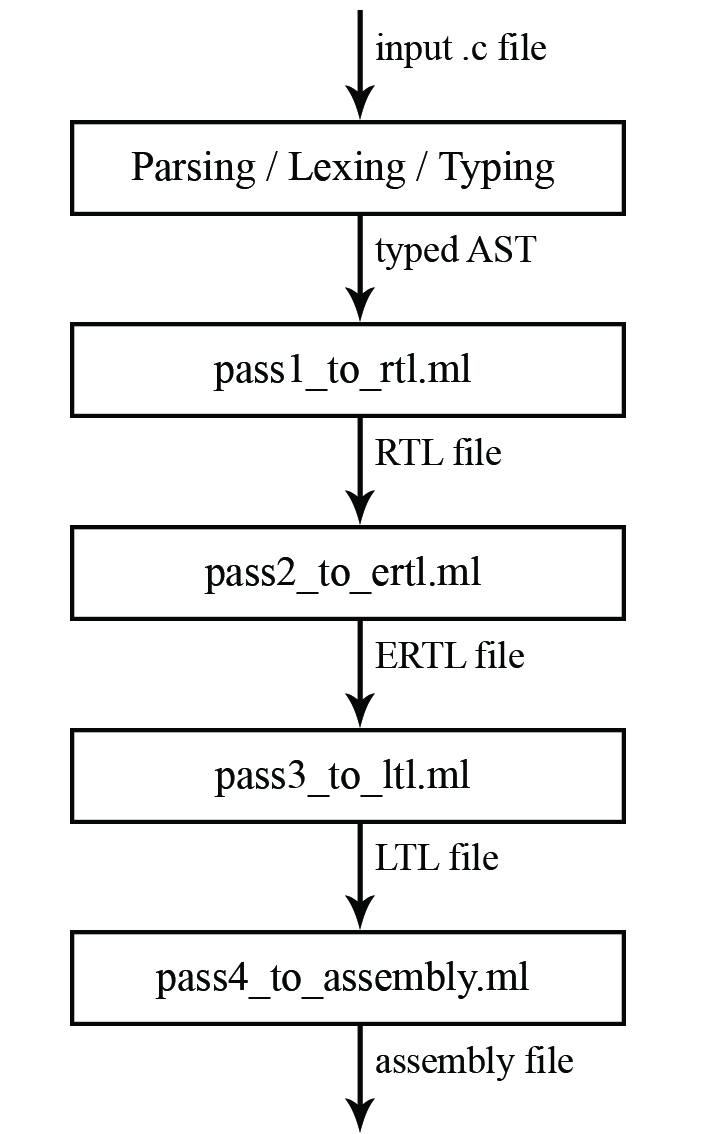
\includegraphics[width=0.3\textwidth]{./images/transformation_flow.jpg}
    \caption{\label{transformations} Les étapes de transformation du code.}
\end{figure}

\end{document}